\chapter{Bisheriger Testablauf}\label{cha:Bisheriger Testablauf}





% Um als führendes Unternehmen in der Stanz-Biegetechnik qualitativ hochwertige Produkte liefern zu können und damit dem guten Ruf der Firma gerecht zu werden, werden die NC-Aggregate seit 2013 mit einem Testverfahren auf einem Prüfstand getestet. Die bis zu diesem Zeitpunkt produzierten geringen Stückzahlen waren zum Testen und auch zum Einlaufen zur Versuchsabteilung nach Halblech gebracht worden.

Um den überdurchschnittlich hohen Anforderungen der Firma Bihler an ihre Produkte gerecht werden zu können, werden die NC-Aggregate seit 2013 mit einem selbst entwickelten Testverfahren auf einem Prüfstand getestet. Die bis zu diesem Zeitpunkt produzierten geringen Stückzahlen waren zum Testen und auch zum Einlaufen zur Versuchsabteilung nach Halblech gebracht worden.

\section{Prüfstand}

Der derzeit zum Testen und auch zum Einlaufen der Aggregate verwendete Prüfstand befindet sich im Werk in Füssen, wo die NACs gefertigt werden und ist der Abteilung Maschinenbau Montage (Unterabteilung Vormontage) zugeordnet.


Der Prüfstand (siehe Abbildung~\ref{fig:Pruefstand}) besteht aus zwei separaten Testmaschinen bzw. Testständen. Hierbei handelt es sich jeweils um einen BM 1500 Würfel mit dazugehörigem Schaltschrank. Zur Versorgung des Prüfstandes ist außerdem eine gemeinsame Kühlanlage vorhanden.


%\begin{comment}
\begin{figure}[H]
\centering
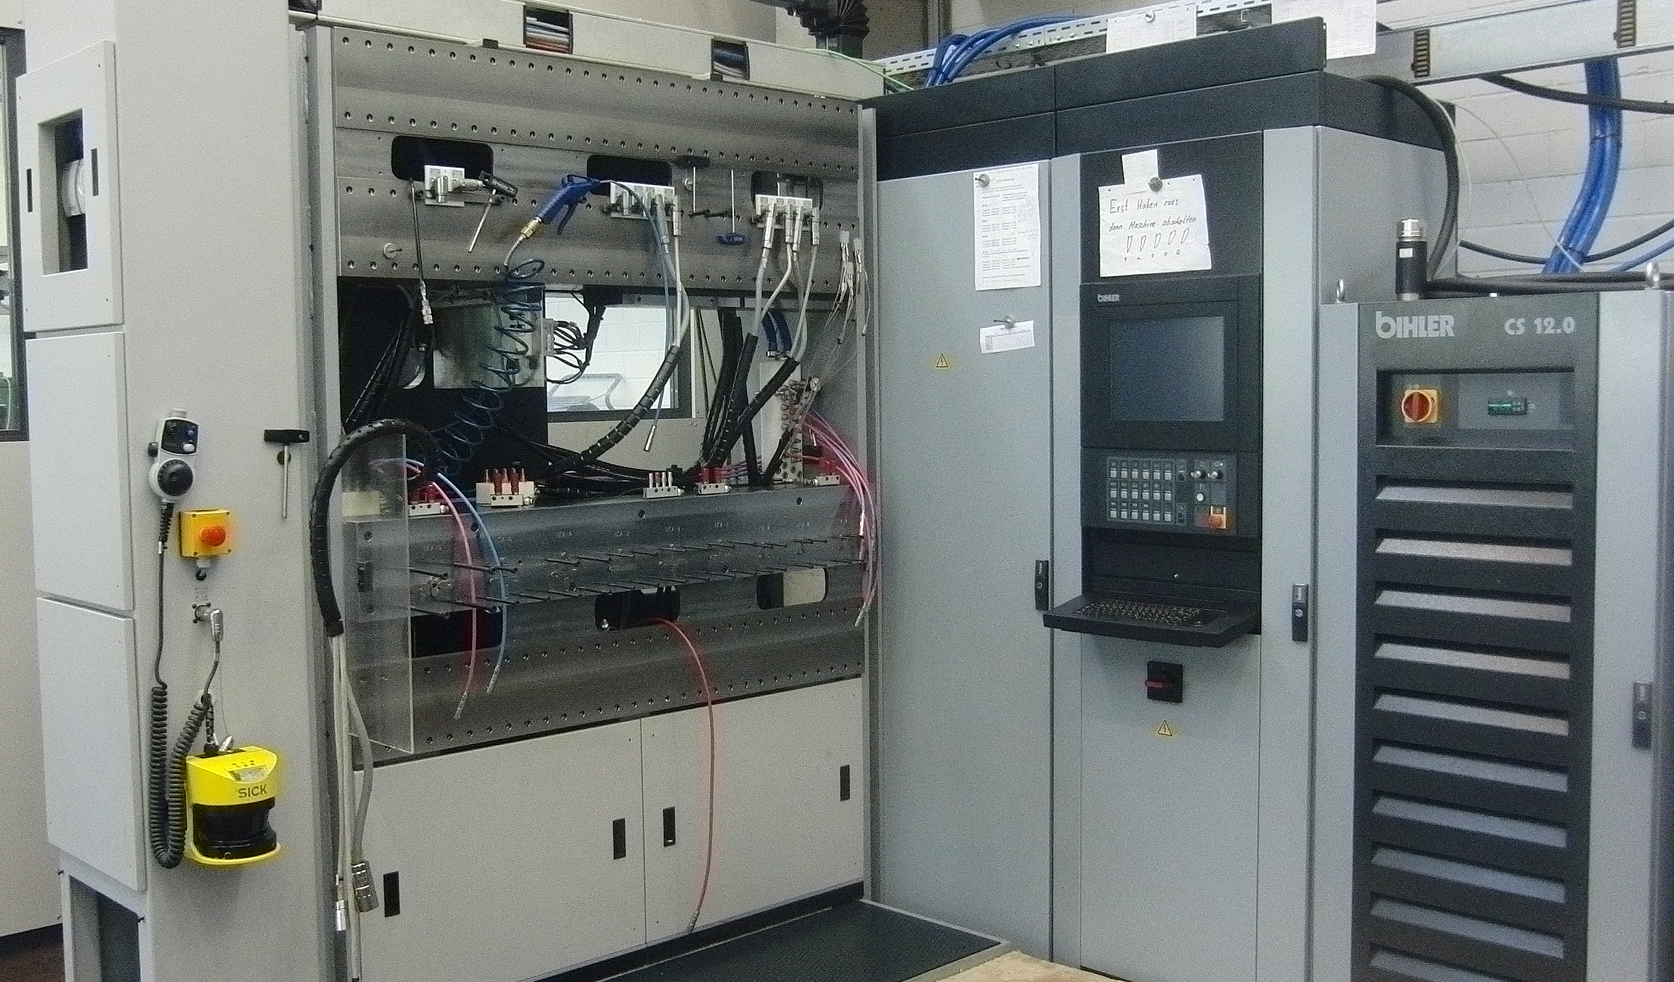
\includegraphics[width=0.9\textwidth]{Teststand_Bild} 
\caption{Teststand NC-Achsen und Kühlanlage} 
\label{fig:Pruefstand}
\end{figure}
%\end{comment}

%\colorbox{orange}{Bild einkommentieren}



Der BM 1500 Würfel dient zur mechanische Befestigung, an dem die NC-Aggregate angeschraubt werden. Zum Aufhängen der schweren NCA 4 und NCA 5 wird der Hallenkran verwendet. In dem Würfel sind die Versorgungsleitungen für Druckluft, Wasser, Schmierung und Strom verlegt. Außerdem ist in dem Würfel das Zentralschmier-System und die Wartungseinheit für die pneumatische Versorgung verbaut.

%\colorbox{yellow}{Zitate für Kühlgerät und regler}

Zum Betreiben der NCAs wird teilweise ein Kühlgerät benötigt. Im Prüfstand ist ein externes Kühlgerät der Firma HYFRA-Industriekühlanlagen GmbH (CS 12.0) vorhanden. Mit diesem kann das Wasser beider Teststände gekühlt werden.

Die Elektronik ist in einem separat aufstellbaren Schaltschrank beheimatet. Zur Anwendung kommt die Steuerungstechnik der Firma B\&R. Als Regler werden die Varianten ACOPOS und ACOPOSmulti verwendet. Je nach eingesetzter Reglergröße kann dieser bestimmte Stromstärken bei konstanter Spannung bereitstellen. Aus diesem Grund kann auf dem älteren der beiden Teststände nur jeweils ein NCA 4 oder ein NCA 5 getestet werden. Auf dem neueren Teststand ist es möglich, 4 NCA 4 oder 4 NCA 5 gleichzeitig zu betreiben. Auf diesem können auch bis zu 5 NCA 2 gleichzeitig getestet werden. Gleichzeitig kann  immer nur ein NCA Typ pro Teststand getestet werden. Neben den Reglern ist im Schaltschrank noch weitere Steuerungs- und Sicherungselektronik wie eine \gls{SPS} verbaut. Auf dem ebenfalls im Schaltschrank verbauten Computer wird die Steuerung betrieben.

Als Steuerung wird die hauseigene VC 1 Steuerung verwendet. Dies ist vorteilhaft, da somit die NCAs mit der auch später im Einsatz eingesetzten Software getestet werden. Nachteilig ist allerdings, dass die Software nicht für Testzwecke sondern für die Massenproduktion vorgesehen ist. Ein Programmieren von Testabläufen und das Abspeichern von Messdaten gestaltet sich deshalb schwierig.




\section{Beschreibung des Testablaufs}\label{cha:Beschreibung_des_Testablaufs}

Mitarbeiter der Abteilung Vormontage oder der Abteilung Serienbetreuung sind damit betraut, den Prüfstand zu betreiben, die entsprechenden Werte zu erfassen, zu dokumentieren und zu bewerten.

Nachdem die NCAs fertig montiert und mit Schmieröl gefüllt sind, werden sie weiter zum Prüfstand zum Testen gebracht.  Da der Rollengewindetrieb eine Einlaufphase benötigt, wie schon in Kapitel~\ref{cha_Besonderheiten_der_Bauelemente} erwähnt, beeinhaltet der bisherige Testablauf gleichzeitig diese Einlaufphase. Wenn die NCAs den Test zufriedenstellend durchlaufen haben, werden sie ins Lager der Logistikabteilung weitergeleitet. Seit zirka 2013 werden die NCAs auf dem Prüfstand mit dem im folgenden beschriebenen Testablauf getestet.


% Innerhalb der Herstellung der NCAs wird der Zeitpunkt nachdem sie montiert und mit Schmieröl gefüllt sind, sind für das Testen verwendet. Sie werden 




Der Prüfablauf der fertig montierten NC-Aggregate setzt sich aus folgenden einzelnen Schritten zusammen.

\begin{enumerate}
 \item Montage der NCAs auf dem Prüfstand 
 \item Anschließen der Versorgungsleitungen (Strom, Motorgeberkabel, Messkopfgeberkabel, Wasser und Schmierung).
 \item Aufsetzen der Temperatursensoren außen auf das Gehäuse 
 \item Einschalten von Maschine und Kühlanlage
 \item Bei NCA 4 Messgeberlineal kalibrieren
 \item Passendes Prüfprogramm laden
 \item Zu prüfende Achsen anwählen und referenzieren
 \item Testablauf starten
 \item Zu messende Werte während des Testablaufes von Hand dokumentieren
 \item Ausschalten der Maschine
 \item Demontage der Aggregate
 \item Weitergabe der geprüften Aggregate
 \item Eintragen der Messwerte in eine Excelarbeitsmappe
\end{enumerate}



\section{Testprogramm}\label{cha:Testprogramm}



Der eigentliche Test der NCAs innerhalb des gesamten Testablaufs besteht darin, dass mit den am Prüfstand angebauten NCAs ein Testprogramm gefahren wird, das innerhalb der Firma Bihler aufgrund der bis dahin gemachten Erfahrungen entwickelt worden ist. Das Testprogramm setzt sich aus verschiedenen Testzyklen zusammen. Jeder Testzyklus besteht aus vielen gleich ablaufenden Hüben, wobei bei jedem Hub die Pinole einmal komplett ein- und ausgefahren wird. 

Jeder Hub wird im Bewegungsprofil Trapez gefahren.  Eine grundlegende Betrachtung zum Trapezprofil ist in Kapitel~\ref{cha:Trapez und Dreiecksprofil} zu finden. Grundsätzlich läuft ein Hub des im Testprogramm gefahrenen Bewegungsprofiles Trapez wie folgt ab:

\begin{enumerate}
 \item Aggregat befindet sich in eingefahrenem Zustand (Weg = 0)
 \item Die Achse wird mit konstanter Beschleunigung beschleunigt
 \item Bei Erreichen einer bestimmten Geschwindigkeit wird die Beschleunigung gestoppt
 \item Die Achse fährt mit konstanter Geschwindigkeit aus
 \item Die Achse wird mit konstanter Beschleunigung gebremst
 \item Die Achse bleibt in ausgefahrenem Zustand stehen (Weg = max)
 \item Die Achse wird mit konstanter Beschleunigung beschleunigt
 \item Bei Erreichen einer bestimmten Geschwindigkeit wird die Beschleunigung gestoppt
 \item Die Achse fährt mit konstanter Geschwindigkeit ein
 \item Die Achse wird mit konstanter Beschleunigung gebremst
 \item Die Achse befindet sich wieder in der Ausgangsposition (Weg = 0)
\end{enumerate}

\begin{figure}
\centering







\begin{tikzpicture}
\begin{groupplot}[
        group style={
            group size=1 by 5,
            xlabels at=edge bottom,
            ylabels at=edge left,
            xticklabels at=edge bottom,
            vertical sep=3pt,
            % vertical sep=40pt
        },
 	width=\textwidth,
 	xmin=0,
 	xmax=1.65,
 	xtick={0,0.2,...,1.8},
 	xlabel={Zeit in $s$},
 	yticklabel style = {font=\small,xshift=0.25ex},
 	,
 	ylabel style = {font=\small,xshift=0.25ex},
    ]
    
\nextgroupplot [
 	no markers,
 	%ymin=0,
    %ymax=5,
  	%title=Einfahrzyklus Drehmomentprofil,
    ylabel={Position in \si{\milli\meter}},
    grid=major,
    ytick={0,30,...,120},
    height=0.23\textheight,
]
    
 	\addplot table[x=Zeit, y=Position]  {graphen/CSV_Daten/Einlaufen_zyklus1_alles.txt};
 	\node[anchor=center] at (axis cs:1.5,105) {A};
    
\nextgroupplot [
 	no markers,
 	%ymin=0,
    %ymax=130,
  	%title=Einfahrzyklus Drehmomentprofil,
    ylabel={Geschwindigkeit in \si{\per\second}},
    grid=major,
    % ytick={-75,-50,...,75},
    height=0.23\textheight,
]
 	\addplot table[x=Zeit, y=Geschwindigkeit]  {graphen/CSV_Daten/Einlaufen_zyklus1_alles.txt};
 	\node[anchor=center] at (axis cs:1.5,10) {B};


\nextgroupplot [
 	no markers,
 	%ymin=0,
    %ymax=130,
  	%title=Einfahrzyklus Drehmomentprofil,
    ylabel={Drehmoment in \si{\newton\meter}},
    grid=major,
    ytick={-10,-5,...,10},
    height=0.23\textheight,
]
 	\addplot table[x=Zeit, y=Drehmoment]  {graphen/CSV_Daten/Einlaufen_zyklus1_alles.txt};
 	\node[anchor=center] at (axis cs:1.5,8) {C};

\nextgroupplot [
 	no markers,
 	%ymin=-0.05,
    %ymax=0.05,
  	%title=Einfahrzyklus Drehmomentprofil,
  	yticklabel style={/pgf/number format/fixed,
                     /pgf/number format/precision=3},
    ylabel={Schleppfehler in \si{\milli\meter}},
    grid=major,
    ytick={-0.01,-0.005,...,0.01},
    height=0.23\textheight,
    scaled y ticks = false,
    tick label style={/pgf/number format/fixed},
]
 	\addplot table[x=Zeit, y=Schleppfehler]  {graphen/CSV_Daten/Einlaufen_zyklus1_alles.txt};
 	\node[anchor=center] at (axis cs:1.5,0.01) {D};
 	
 	
\nextgroupplot [,
 	no markers,
 	ymin=-0.035,
    ymax=0.035,
  	%title=Einfahrzyklus Drehmomentprofil,
    ylabel={Positionsdifferenz in \si{\milli\meter}},
    grid=major,
    ytick={-0.03,-0.02,...,0.03},
    height=0.23\textheight,
    scaled y ticks = false,
    tick label style={/pgf/number format/fixed},
]
 	\addplot table[x=Zeit, y=Positionsdifferenz]  {graphen/CSV_Daten/Einlaufen_zyklus1_alles.txt};
 	\node[anchor=center] at (axis cs:1.5,0.02) {E};

\end{groupplot}

%\draw (my plots c1r1.east) circle (3pt) node {East};


\end{tikzpicture}
\caption{Kennkurven (A bis E) während des Testlaufes (Zyklus 1 NCA 4 mit p = 10) für einen Hub}
\label{fig:Einlaufen_zyklus1_alles}
\end{figure}


Die graphische Darstellung eines Hubes veranschaulichen die Abbildungen~\ref{fig:Einlaufen_zyklus1_alles}~A bis E. In ihnen wird ein Hub des Testlaufes (Zyklus 1 NCA 4 mit p = 10) mit verschiedenen Messwerten dargestellt. Abbildung~\ref{fig:Einlaufen_zyklus1_alles}~A stellt die Position des NCAs dar. In Abbildung~\ref{fig:Einlaufen_zyklus1_alles}~B ist die Geschwindigkeit zu erkennen. Diese beiden Kurven sind für ein Trapezprofil typisch. Ergänzende Messwerte sind in den Abbildungen~\ref{fig:Einlaufen_zyklus1_alles}~C bis E aufgeführt. Nähere Erklärungen zu den Messwerten Schleppfehler und Positionsdifferenz sind in Kapitel~\ref{cha: Messgroessen Stufenprofil} zu finden. 


\begin{table}[ht]
\centering






\begin{tabular}{ccccc}\toprule
 & Bewegungsgesetz & Übergangswinkel & Motordrehzahl & Geschwindigkeit  \\
 & & $^\circ$ & U/min & mm/s  \\
\midrule
Zyklus 1 & Trapez & 180 & 1000 & 166,7\\
Zyklus 2 & Trapez & 180 & 2000 & 333 \\
Zyklus 3 & Trapez & 180 & 3000 & 500 \\
Zyklus 4 & Trapez & 180 & 1000 & 166,7 \\
\bottomrule
\end{tabular}

\smallskip

\begin{tabular}{cccccc}
 & Beschleunigung & Beschleunigung & Maschinendrehzahl &  Dauer & Hub \\
 & U/s$^2$ & mm/s$^2$ & U/min & min & mm \\
\midrule
Zyklus 1 & 9000 & 1500 & 103 & 30 & 120 \\
Zyklus 2 & 9000 & 1500 & 103 & 30 & 120 \\
Zyklus 3 & 9000 & 1500 & 103 & 30 & 120 \\
Zyklus 4 & 9000 & 1500 & 103 & 5 & 120 \\
\bottomrule
\end{tabular}



\caption{Testzyklen (NCA 4) p=10 (aus Programm ausgelesen)}
\label{Einlauf_Zyklen}
\end{table}




\begin{table}[h]
\centering
\begin{tabular}{ccc}\toprule
& Zeit je Hub in s & Anzahl Hübe \\
\midrule
Zyklus 1 & 1,59 & 1129 \\
Zyklus 2 & 0,90 & 2005 \\
Zyklus 3 & 0,68 & 2647 \\
Zyklus 4 & 1,59 & 188 \\
\bottomrule
\end{tabular}
\caption{Anzahl der Hübe je Zyklus (gemessen)}
\label{Einlauf_Zyklen_Anzahl}
\end{table}


Ein Testzyklus besteht aus der Wiederholung eines genau definierten Hubes über eine bestimmten Zeitraum hinweg. Die Dauer für die einzelnen Zyklen kann man der Tabelle~\ref{Einlauf_Zyklen} entnehmen. Diese Zeiträume sind für die Testprogramme aller NCA Varianten gleich. Die Parameter für die einzelnen Hübe können beispielhaft für ein NCA 4 p=10 der Tabelle~\ref{Einlauf_Zyklen} entnommen werden. Allerdings sind die Ruhezeiten in den Endpositionen nicht definiert. Die Anzahl der Hübe ist nicht genau definiert, sondern wurde vom Programmierer der Testprogramme willkürlich festgelegt. Somit ist die Anzahl der Hübe, die innerhalb eines Testzyklus ablaufen, nicht genau festgelegt oder errechenbar. Für ein NCA 4 p=10 wurde im Rahmen dieser Arbeit die Zeit, die für einen Hub benötigt wird, gemessen und daraus die Anzahl der während einer Zyklusdauer auftretenden Hübe berechnet. Die Anzahl der Hübe und die Dauer eines Hubes für die verschiedenen Zyklen kann der Tabelle~\ref{Einlauf_Zyklen_Anzahl} entnommen werden.






Das Testprogramm für eine bestimmte NCA Variante setzt sich aus 4 verschiedenen Testzyklen zusammen. Die Parameter der einzelnen Zyklen können der Tabelle~\ref{Einlauf_Zyklen} entnommen werden. Jeder der ersten drei Zyklen dauert eine halbe Stunde. Der 4. Zyklus dauert 5 Minuten. Früher dauerten die ersten drei Zyklen jeweils 2 Stunden. Da jedoch auch jeweils eine halbe Stunde pro Zyklus für das Einlaufen des Aggregates ausreicht, konnten diese Zeiten auf die nun verwendeten 30 Minuten verkürzt werden.



Die Beschleunigungen bleiben bei allen Testzyklen gleich. Nur die Geschwindigkeit wird während der ersten drei Zyklen von Testzyklus zu Testzyklus erhöht. (siehe Tabelle~\ref{Einlauf_Zyklen} und Abbildung~\ref{Einfahrzyklus_Geschwindigkeitsprofil}) Durch die höhere Geschwindigkeit verkürzt sich die Zeit für einen Hub (siehe Abbildung~\ref{Einfahrzyklus_Wegprofil}). Der am Ende gefahrene 4. Zyklus ist mit 5 Minuten wesentlich kürzer als die vorhergehenden Zyklen mit 30 Minuten. Er wird mit den gleichen Parametern gefahren, wie der 1. Zyklus, das Ein- und Ausfahren der Pinole wird deshalb jedoch weniger oft wiederholt.  Auf diese Weise prüft man das Aggregat nach dem Einlaufen. Die Verwendung des Trapezprofils ist vor allem mit dem Funktionsumfang der VC 1 Steuerung zu begründen.






\begin{figure}[H]
\begin{tikzpicture}
 \begin{axis}[
 	no markers,
 	ymin=0,
    xmin=0,
 	width=\textwidth,height=0.2\textheight,
  	%title=Einfahrzyklus Wegprofil,
    xlabel={Zeit in s},
    ylabel={Weg in mm},
    grid=major,
    legend entries={Zyklus 1,Zyklus 2,Zyklus 3},
    enlarge x limits=0.01,
]
 	\addplot table[x=Zeit1, y=Lauf1mm]  {graphen/Positionsprofil_Einlaufen.csv};
 	\addplot table[x=Zeit2, y=Lauf2mm]  {graphen/Positionsprofil_Einlaufen.csv};
 	\addplot table[x=Zeit3, y=Lauf3mm]  {graphen/Positionsprofil_Einlaufen.csv};
 \end{axis}
\end{tikzpicture}
\caption{Einfahrzyklus Wegprofil (für jeden Zyklus ist ein Hub dargestellt)}
\label{Einfahrzyklus_Wegprofil}
\end{figure}



\begin{figure}[H]
\begin{tikzpicture}
 \begin{axis}[
 	no markers,
 	%ymin=0,
    xmin=0,
 	width=\textwidth,height=0.2\textheight,
  	%title=Einfahrzyklus Geschwindigkeitsprofil,
    xlabel={Zeit in s},
    ylabel={Geschwindigkeit in mm/s},
    grid=major,
    legend entries={Zyklus 1,Zyklus 2,Zyklus 3},
    enlarge x limits=0.01,
]
 	\addplot table[x=Zeit1, y=Lauf1Units]  {graphen/Geschwindigkeitsprofil_Einlaufen.csv};
 	\addplot table[x=Zeit2, y=Lauf2Units]  {graphen/Geschwindigkeitsprofil_Einlaufen.csv};
 	\addplot table[x=Zeit3, y=Lauf3Units]  {graphen/Geschwindigkeitsprofil_Einlaufen.csv};
 \end{axis}
\end{tikzpicture}
\caption{Einfahrzyklus Geschwindigkeitsprofil (für jeden Zyklus ist ein Hub dargestellt)}
\label{Einfahrzyklus_Geschwindigkeitsprofil}
\end{figure}





\section{Ermittelte Messgrößen}\label{cha:Ermittelte_Messwerte}

Wie in Kapitel~\ref{cha:Beschreibung_des_Testablaufs} beschrieben, werden die während des Testablaufes gemessenen Werte dokumentiert. Bei diesen gemessenen Werten handelt es sich je Testlauf und Aggregat um:


%Es werden folgende Werte je Testlauf und Aggregat gemessen:
\begin{itemize}
 \item Maximale Stromstärke bei konstanter Geschwindigkeit beim Ausfahren (bei allen 4 Zyklen)
 \item Temperatur von 3 außen auf dem Gehäuse aufgebrachten Sensoren (bei den ersten 3 Zyklen)
 \item Motortemperatur (bei den ersten 3 Zyklen)
\end{itemize}

% Man will mit diesen Werten gravierenden Problemen der einzelnen NC-Aggregate in der Serienfertigung auf die Spur kommen.

% Eine genauere Erklärung zu den Messmethoden und den erfassten Werten erfolgt in den weiteren Unterkapiteln.

\subsection{Stromstärke}\label{ch:Ermittelte_Messwerte_Stromstaerke}

Zur Ermittlung der maximalen Stromstärke zeichnet der Regler innerhalb des Testprogramms während aller Testzyklen bei jedem Hub die Stromstärke beim Aus- und Einfahren auf. Es wird angenommen, dass Stromstärke und Drehmoment im Zusammenhang mit dem Testlauf proportional sind. Hierzu wird  durch den Elektromotorenhersteller eine entsprechende Drehmomentkonstante angegeben. Mit dieser kann man die Stromstärke in das Drehmoment umrechnen. Bei allen nachfolgenden Messungen wurde jeweils nur die Stromstärke gemessen, nicht das Drehmoment.

%\colorbox{yellow}{Zitat für Datenblatt einfügen}

Die Messung der Stromstärke beginnt, sobald der Beschleunigungsvorgang beendet ist. Die Messung wird mit Beginn des Abbremsvorganges beendet. Im Messbereich wird der höchste Wert ermittelt. Dieser wird für jeden Hub aufgezeichnet und über die VC 1 Oberfläche angezeigt. Der höchste aller am Ende eines Testzyklus gemessenen Werte wird dokumentiert. In der Abbildung~\ref{fig:Ermittlung des Drehmoment Kennwertes im Einfahrzyklus} ist beispielhaft das gemessenen Drehmoment während eines Hubes dargestellt und der Messbereich gekennzeichnet, aus dem der als Messwert verwendete Höchstwert ermittelt wird. Die Spitzen stellen die Be- und Entschleunigungsvorgänge während des Hubes dar.

% Die Umrechnung von Stromstärke auf Drehmoment erfolgt über die sogenannte Drehmomentkonstante. Somit sind Stromstärke und Drehmoment in ihren qualitativen Aussagen als äquivalent anzusehen. Physikalisch ist dies allerdings nicht ganz korrekt, da aufgrund der Drehmomentkonstanten von einem direkt proportionalen Verhalten ausgegangen wird, das insbesondere in den Grenzbereichen nicht vorhanden ist.



\begin{figure}[H]
\begin{tikzpicture}
 \begin{axis}[
 	no markers,
 	%ymin=0,
    xmin=0,
 	width=\textwidth,height=0.4\textheight,
  	%title=Einfahrzyklus Drehmomentprofil,
    xlabel={Zeit in s},
    ylabel={Drehmoment in Nm},
    grid=major,
    %legend entries={Zyklus 1,Zyklus 2,Zyklus 3},
    enlarge x limits=0.01,
]
 	\addplot table[x=Zeit1, y=Lauf1Units]  {graphen/Drehmoment_Einlaufen.csv};
 	\draw[help lines, dashed](current axis.south-|{axis cs:0.088,1})%
       --(current axis.north-|{axis cs:0.088,1});%node[left,pos=0.7]{$76$};
    \draw[help lines, dashed](current axis.south-|{axis cs:0.77,1})%
       --(current axis.north-|{axis cs:0.77,1});%node[right,pos=0.7]{$89$};
    \draw [<->] (axis cs: 0.088, 6) -- (axis cs: 0.77, 6) node[midway, above] {Messbereich};
    \draw [thin, Bihler2] (current axis.west|-{axis cs: 1, 0.934}) -- (axis cs: 0.77, 0.934) node[midway, above] {Messwert: \SI{0.93}{\newton\meter}};
 \end{axis}
\end{tikzpicture}
\caption{Ermittlung des Drehmoment- bzw. Stromstärke-Kennwertes während eines Hubes}
\label{fig:Ermittlung des Drehmoment Kennwertes im Einfahrzyklus}
\end{figure}


\clearpage

In Abbildung~\ref{fig:Einfahrzyklus_Drehmomentprofil} sind die Drehmomentkurven je eines Hubes von den ersten drei Testzyklen aufgezeichnet. Wie erwartet, werden im Bereich der konstanten Geschwindigkeit die Drehmomente umso größer, je höher die Geschwindigkeit ist (vgl. Kapitel~\ref{cha:Testprogramm}). Die Spitzen stellen wiederum die Be- und Entschleunigungsvorgänge während jedes Hubes dar.

\begin{figure}[H]
\begin{tikzpicture}
 \begin{axis}[
 	no markers,
 	%ymin=0,
    xmin=0,
 	width=\textwidth,height=0.4\textheight,
  	%title=Einfahrzyklus Drehmomentprofil,
    xlabel={Zeit in s},
    ylabel={Drehmoment in Nm},
    grid=major,
    legend entries={Zyklus 1,Zyklus 2,Zyklus 3},
    enlarge x limits=0.01,
]
 	\addplot table[x=Zeit1, y=Lauf1Units]  {graphen/Drehmoment_Einlaufen.csv};
 	\addplot table[x=Zeit2, y=Lauf2Units]  {graphen/Drehmoment_Einlaufen.csv};
 	\addplot table[x=Zeit3, y=Lauf3Units]  {graphen/Drehmoment_Einlaufen.csv};
 \end{axis}
\end{tikzpicture}
\caption{Drehmoment- bzw. Stromstärkeprofile je eines Hubes der ersten drei Testzyklen}
\label{fig:Einfahrzyklus_Drehmomentprofil}
\end{figure}

\subsection{Temperatur an der Außenseite der NC-Aggregate} \label{cha:Temperatur_an_der_Aussenseite_des_NCA}








Mit der Messung der Temperatur will man erkennen, ob sich die Temperatur am Lager, am Gehäuse oder am Abstreifer übermäßig erhöht. Pro Aggregat werden für den Testlauf drei Temperatursensoren PT100 außen am Gehäuse angebracht. Ihre Lagen können der Abbildung~\ref{fig:Position_der_Temperatursensoren} entnommen werden. Die Auswertung der Temperatursensoren erfolgt dabei über die Elektronik der VC 1 Steuerung. Sie werden mit Magneten in ihrer Position gehalten. Jede Minute wird je ein Messwert pro Sensor für jeden der drei ersten Testzyklen aufgenommen und von der VC 1 Steuerung angezeigt. Als Ergebnis der Messung wird je Sensor jeweils der höchste Messwert pro 30 minütigem Testzyklus notiert. Dies ergibt somit 9 Messwerte.

\clearpage


% Die Lage der Temperatursensoren können der Abbildung~\ref{fig:Position_der_Temperatursensoren} entnommen werden. Die Sensoren sind vom Typ PT100. Sie werden mit Magneten in ihrer Position gehalten. Jede Minute wird je ein Messwert pro Sensor aufgenommen und abgespeichert. Als Ergebnis des Testablaufes wird jeweils der höchste Messwert am Ende der ersten drei Zyklen notiert. Man will mit dieser Messung erkennen, ob sich die Temperatur am Lager, am Gehäuse oder am Abstreifer übermäßig erhöht. 

%\begin{figure}[H]
%\centering
%\includegraphics[trim=5cm 5cm 5cm 5cm, clip=true, height=0.3\textwidth, angle=270]{Temperatursensoren_reales_Bild}
%\caption{NCA 5 Bereit zum Testlauf}
%\label{fig:NCA_5_Bereit_zum_Testlauf}
%\end{figure}


\begin{figure}[H]
\centering
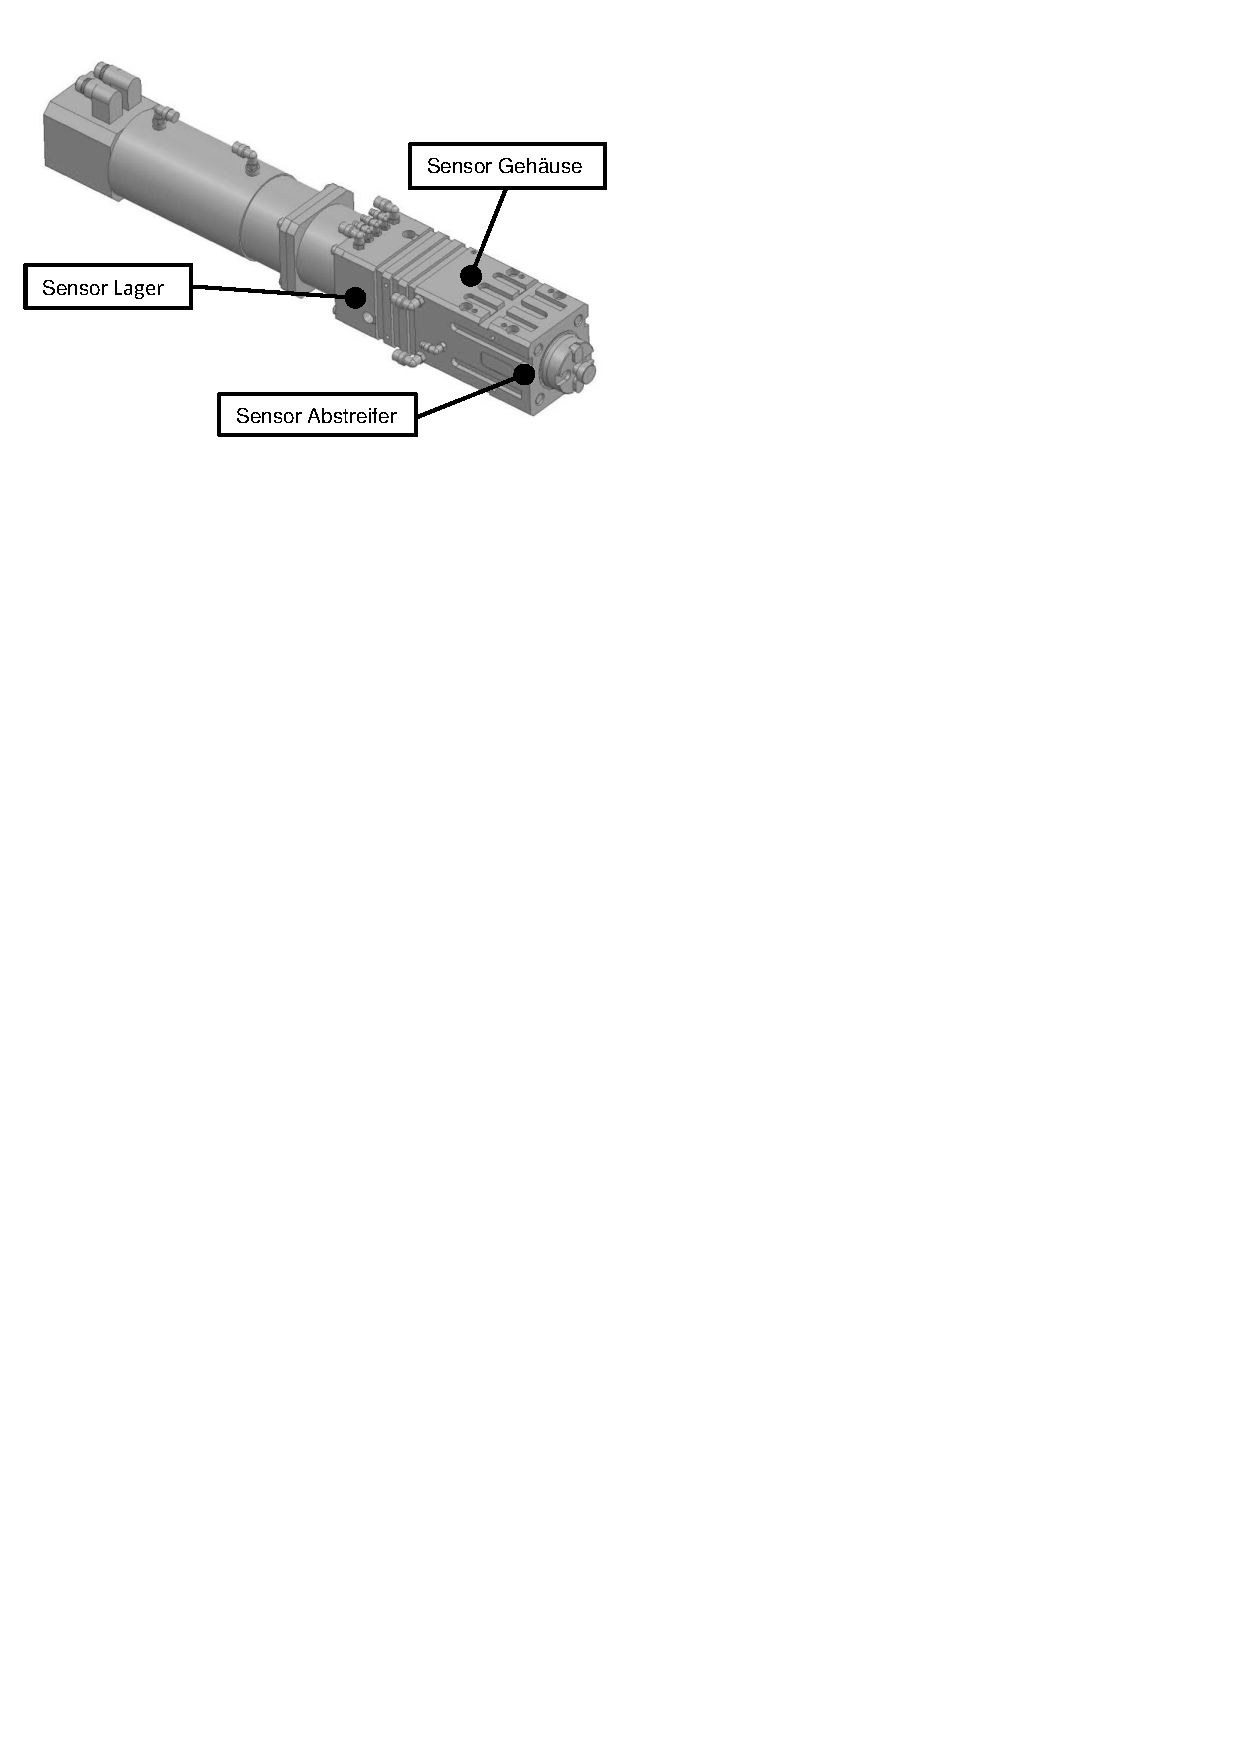
\includegraphics[width=0.7\textwidth]{NCA4_Positionen_Temperatursensoren} % Bild der Temperatursensoren
\caption{Position der Temperatursensoren} 
\label{fig:Position_der_Temperatursensoren}
\end{figure}

Der Verlauf der gemessenen Temperatur für das gesamte Testprogramm ist in Abbildung~\ref{fig:Einlauf_Temperaturanzeige} zu sehen.  Durch die Kühlung des Aggregates ist der Temperaturanstieg gering. Die der Abbildung zugrunde liegenden Werte werden im normalen Testlauf zwar in der gleichen Form erfasst wie in der Abbildung dargestellt, aber nicht abgespeichert. Deshalb werden sie im Rahmen dieser Arbeit gesondert aufgezeichnet, um den Temperaturverlauf darstellen zu können. Bei der hier gezeigten Messung wird somit jede Minute ein Messwert mit einer nominalen Auflösung von einem Zehntel Kelvin aufgezeichnet.

\begin{figure}[H]
\begin{tikzpicture}
 \begin{axis}[
 	no markers,
 	% ymin=0,
    xmin=0,
    xmax=96,
 	width=\textwidth,height=0.4\textheight,
  	%title=Einfahrzyklus Drehmomentprofil,
    xlabel={Zeit in min},
    ylabel={Temperatur in $^\circ$C},
    grid=major,
    legend entries={Sensor Lager,Sensor Gehäuse,Sensor Abstreifer},
    legend pos=south east,
    %enlarge x limits=0.01,
]
 	\addplot table[x=Punkte:, y=Temperatursensor1]  {graphen/CSV_Daten/Trendanzeige_Temperatur_Aggregat38207.txt};
 	\addplot table[x=Punkte:, y=Temperatursensor2]  {graphen/CSV_Daten/Trendanzeige_Temperatur_Aggregat38207.txt};
 	\addplot table[x=Punkte:, y=Temperatursensor3]  {graphen/CSV_Daten/Trendanzeige_Temperatur_Aggregat38207.txt};
 \end{axis}
\end{tikzpicture}

% StromLauf1
\caption{Temperaturverlauf an der Außenseite während des Testprogramms bei dem Aggregat mit der Seriennummer 38207}
\label{fig:Einlauf_Temperaturanzeige}
\end{figure}


\subsection{Motortemperatur} \label{cha:Einlaufen_Motortemperatur}

Der Motor besitzt einen eingebauten Temperatursensor. Dieser Wert wird von der Steuerung ausgelesen und kann im Display der Steuerung als Zahlenwert dargestellt werden. Als Messwert wird hierbei der höchste Wert während der letzten Minuten der ersten drei Zyklen aufgezeichnet. 

\section{Auswertung des bisherigen Testablaufs}

Die während der Tests der Aggregate erfassten Daten wurden vom Betrieb bisher nicht ausgewertet. Eine Auswertung wird im Rahmen dieser Arbeit, wie nachfolgend dargestellt, angestrebt. Dabei wird nachfolgend analysiert, ob es sinnvoll ist, diese Messungen durchzuführen und diese Daten zu erfassen, wie aussagekräftig sie sind und welche Rückschlüsse auf die Funktionsfähigkeit der NCAs aus dem derzeitigen Testprogramm gezogen werden können. So werden die Daten für Stromstärke, Motortemperatur und die Temperatur an der Außenseite der NC-Aggregate herangezogen, um das momentane Testverfahren zu analysieren.

Um eine genügend große Anzahl an Messwerten zu erhalten, erfolgt die Auswertung nur aufgrund der Größentypen der NCAs (NCA 2 - 4) und nicht nach dem wesentlich aussagekräftigeren Baustand, der anhand der Artikelnummer ermittelt werden kann. (vergleiche Anhang~\ref{cha_Anhang_4})



\subsection{Stromstärke}

Ein mögliches Auswertungskriterium der bisher erfassten Daten ist die Stromaufnahme des Motors. Diese wird vom Regler erfasst und, wie unter Kapitel~\ref{ch:Ermittelte_Messwerte_Stromstaerke} beschrieben, aufgezeichnet.

Für die Auswertung werden die Messwerte aller seit 2013 getesteten NCAs in Histogrammen dargestellt. Die Klassenbreite beträgt hierbei 0,1 A. Von der üblichen Darstellungsweise in Balkenform wird abgewichen, um die Verschiebung von Zyklus zu Zyklus leichter erkennen zu können.


% Für die Auswertung werden die Messwerte aller seit 2013 getesteten NCAs in Ampere von zwei Stellen nach dem Komma auf eine Stelle nach dem Komma gerundet. Dann wird jeweils die Anzahl der Aggregate ermittelt, die die gleiche Stromaufnahme besitzen. Zur besseren Anschaulichkeit werden die Punkte miteinander verbunden. Von der üblichen Darstellungsweise als Histogramm wird somit abgewichen, um die Verschiebung 

Dies ergibt somit für die NCA2 - NCA5 jeweils 4 Kurven, je eine pro Testzyklus. Diese sind in den Abbildungen ~\ref{fig:Stromaufnahme_NCA_2}, ~\ref{fig:Stromaufnahme_NCA_3}, ~\ref{fig:Stromaufnahme_NCA_4} und ~\ref{fig:Stromaufnahme_NCA_5} zu finden. Wie zu erwarten, steigt die benötigte Stromstärke bei zunehmender Geschwindigkeit. Manche Werte scheinen nicht besonders plausibel (vergleiche NCA 3, Zyklus 3 in Abbildung ~\ref{fig:Stromaufnahme_NCA_3}). Dies könnte zum Beispiel durch eine fehlerhafte Messung verursacht sein.

In allen vier Abbildungen ist der Rückgang der benötigten Stromstärke von Zyklus 1 auf Zyklus 4, der zur Kontrolle dient, zu erkennen. Diese bei gleichen Parametern gemessenen Werte spiegeln den Einlaufvorgang des Rollengewindetriebes wider. Nach dem Einlaufen wird somit für die gleiche Verfahrbewegung weniger Strom und somit weniger Energie benötigt. Dadurch lässt sich zeigen, dass ein erfolgreiches Einlaufen des Rollengewindetriebes stattgefunden hat.

Grundsätzlich ist mit der Messung der Stromstärke somit eine Schwergängigkeit der Aggregate feststellbar. Entsprechend hohe Werte würden dazu Anlass geben, das Aggregat nochmals genauer zu betrachten. Hierzu sind allerdings keine Fälle dokumentiert.

Bei den NCA 4 Aggregaten sind für jeden Zyklus zwei voneinander getrennte Spitzen in den Graphen zu erkennen. (vgl. Abbildung~\ref{fig:Stromaufnahme_NCA_4}) Bei einer genaueren Betrachtung der Daten ist dies auf eine konstruktive Änderung der NCA 4 Achsen zurückzuführen. Zukünftig sollte deshalb eine getrennte Analyse der unterschiedlichen Bautypen erfolgen.


\begin{figure}[H]
\begin{tikzpicture}
 \begin{axis}[
 	ymin=0,
    xmin=0,
 	width=\textwidth,height=0.26\textheight,
  	%title=Stromaufnahme NCA 2,
    xlabel={Stromstärke in A},
    ylabel={Anzahl der Aggregate},
    grid=major,
    legend entries={Zyklus 1,Zyklus 2,Zyklus 3,Zyklus 4},
    enlarge x limits=0.01,
]
 	\addplot+[mark=*] table[x=Ampere, y=Zyklus1]  {graphen/Stromauswertung_Einfahrzyklus_NCA2.csv};
    \addplot+[mark=x] table[x=Ampere, y=Zyklus2] {graphen/Stromauswertung_Einfahrzyklus_NCA2.csv};
    \addplot+[mark=+] table[x=Ampere, y=Zyklus3] {graphen/Stromauswertung_Einfahrzyklus_NCA2.csv};
    \addplot+[mark=asterisk] table[x=Ampere, y=Zyklus4] {graphen/Stromauswertung_Einfahrzyklus_NCA2.csv};
 \end{axis}
\end{tikzpicture}
\caption{Anzahl der NCA 2 mit ihrer jeweiligen maximalen Stromstärke in den 4 Testzyklen}
\label{fig:Stromaufnahme_NCA_2}
\end{figure}



\begin{figure}[H]
\begin{tikzpicture}
 \begin{axis}[
 	ymin=0,
    xmin=0,
 	width=\textwidth,height=0.26\textheight,
  	%title=Stromaufnahme NCA 3,
    xlabel={Stromstärke in A},
    ylabel={Anzahl der Aggregate},
    grid=major,
    legend entries={Zyklus 1,Zyklus 2,Zyklus 3,Zyklus 4},
    enlarge x limits=0.01,
]
 	\addplot+[mark=*] table[x=Ampere, y=Zyklus1]  {graphen/Stromauswertung_Einfahrzyklus_NCA3.csv};
    \addplot+[mark=x] table[x=Ampere, y=Zyklus2] {graphen/Stromauswertung_Einfahrzyklus_NCA3.csv};
    \addplot+[mark=+] table[x=Ampere, y=Zyklus3] {graphen/Stromauswertung_Einfahrzyklus_NCA3.csv};
    \addplot+[mark=asterisk] table[x=Ampere, y=Zyklus4] {graphen/Stromauswertung_Einfahrzyklus_NCA3.csv};
 \end{axis}
\end{tikzpicture}
\caption{Anzahl der NCA 3 mit ihrer jeweiligen maximalen Stromstärke in den 4 Testzyklen}
\label{fig:Stromaufnahme_NCA_3}
\end{figure}



\begin{figure}[H]
\begin{tikzpicture}
 \begin{axis}[
 	ymin=0,
    xmin=0,
 	width=\textwidth,height=0.26\textheight,
  	%title=Stromaufnahme NCA 4,
    xlabel={Stromstärke in A},
    ylabel={Anzahl der Aggregate},
    grid=major,
    legend entries={Zyklus 1,Zyklus 2,Zyklus 3,Zyklus 4},
    enlarge x limits=0.01,
]
 	\addplot+[mark=*] table[x=Ampere, y=Zyklus1]  {graphen/Stromauswertung_Einfahrzyklus_NCA4.csv};
    \addplot+[mark=x] table[x=Ampere, y=Zyklus2] {graphen/Stromauswertung_Einfahrzyklus_NCA4.csv};
    \addplot+[mark=+] table[x=Ampere, y=Zyklus3] {graphen/Stromauswertung_Einfahrzyklus_NCA4.csv};
    \addplot+[mark=asterisk] table[x=Ampere, y=Zyklus4] {graphen/Stromauswertung_Einfahrzyklus_NCA4.csv};
 \end{axis}
\end{tikzpicture}
\caption{Anzahl der NCA 4 mit ihrer jeweiligen maximalen Stromstärke in den 4 Testzyklen}
\label{fig:Stromaufnahme_NCA_4}
\end{figure}



\begin{figure}[H]
\begin{tikzpicture}
 \begin{axis}[
 	ymin=0,
    xmin=0,
 	width=\textwidth,height=0.26\textheight,
  	%title=Stromaufnahme NCA 5,
    xlabel={Stromstärke in A},
    ylabel={Anzahl der Aggregate},
    grid=major,
    legend entries={Zyklus 1,Zyklus 2,Zyklus 3,Zyklus 4},
    enlarge x limits=0.01,
]
 	\addplot+[mark=*] table[x=Ampere, y=Zyklus1]  {graphen/Stromauswertung_Einfahrzyklus_NCA5.csv};
    \addplot+[mark=x] table[x=Ampere, y=Zyklus2] {graphen/Stromauswertung_Einfahrzyklus_NCA5.csv};
    \addplot+[mark=+] table[x=Ampere, y=Zyklus3] {graphen/Stromauswertung_Einfahrzyklus_NCA5.csv};
    \addplot+[mark=asterisk] table[x=Ampere, y=Zyklus4] {graphen/Stromauswertung_Einfahrzyklus_NCA5.csv};
 \end{axis}
\end{tikzpicture}
\caption{Anzahl der NCA 5 mit ihrer jeweiligen maximalen Stromstärke in den 4 Testzyklen}
\label{fig:Stromaufnahme_NCA_5}
\end{figure}




\subsection{Temperatur}



Die Motortemperatur wird durch die Kühlung auf wenige Kelvin konstant gehalten. Somit ist eine aussagekräftige Auswertung dieser Messung nicht möglich.

Auch bei den extern angebrachten Temperatursensoren werden mögliche Unterschiede zwischen den einzelnen Aggregaten durch die Kühlung minimiert. Das Aggregat wird somit auf annähernd konstanter Temperatur gehalten, indem durch einen eventuellen Fehler wesentlich mehr Energie an das Kühlwasser abgegeben werden würde. Außerdem wird die Umgebungstemperatur bei der derzeitigen Datenerfassung nicht berücksichtigt. Dies bedeutet, dass zwei Messungen dieselbe Temperatur anzeigen können, obwohl sich ein Aggregat aufgrund eines Fehlers stärker als ein anderes Aggregat erwärmt hat.



Da die einzelnen aufgezeichneten absoluten Temperaturwerte nicht vergleichbar sind, gibt es keine Möglichkeit, sie aussagefähig auszuwerten.





\section{Analyse des bisherigen Testablaufes} \label{ch:Kritik_Testlauf}






%Verschiedene relevante Faktoren werden durch den momentanen Testablauf erfasst.

Die grundsätzliche Funktionsfähigkeit der NCAs wird dadurch festgestellt, dass im Teststand das erste Mal versucht wird, das Aggregat mithilfe ihrer Steuerung in Gang zu setzen. Dadurch kann man feststellen, ob die Steuerung alle elektrischen Komponenten ansprechen kann, ob sich der Motor wie erwartet ansteuern lässt, das Messlineal verarbeitbare Werte zurückgibt und keines der angeschlossenen Komponenten einen Fehler an die Steuerung meldet. Dabei sind folgende Verbesserungspotentiale denkbar:

\begin{itemize}
    \item Bis jetzt gibt es für alle während der Testphase der NCAs erfassten  Messwerte keine Toleranzen oder Nennwerte. Dies bedeutet, dass zwar die Messwerte bei jedem Aggregat aufgezeichnet werden, es aber aufgrund dieser Werte zu keinen Entscheidungen darüber kommt, ob ein Aggregat voll funktionstüchtig ist oder nicht. 
    \item Aggregate bestehen nur nach subjektiven Kriterien der mit dem Test befassten Mitarbeiter den Testlauf nicht.
    \item Es werden nur sehr grobe Fehler gefunden, z.B. wenn sich das Aggregat nicht über die Steuerung betreiben lässt oder ungewöhnliche Geräusche emittiert. Aus diesem Grund ist mit dem Ende des Testlaufes kein einheitlicher Standard für die Qualität der Achsen sichergestellt. 
    \item Die erkannten Fehler werden nicht durchgängig mitprotokolliert, um daraus eine Fehlerdatenbank aufbauen zu können. Deswegen ist das Wissen über die Fehler sehr stark von den einzelnen Mitarbeitern abhängig und es ist schwierig, bekannte Probleme gezielt abzustellen. 
    \item Außerdem beginnt die Suche nach der Ursache von eigentlich bekannten Problemen immer wieder aufs neue, da unternommene Versuche der Ursachenfindung nicht strukturiert dokumentiert werden.
    \item Da die Aufzeichnung der Messwerte für Motortemperatur, Aggregat-Außenseiten-Tem\-pe\-ra\-tur und Stromstärke per Hand und nicht automatisiert erfolgt, ist die Aufnahme der Messwerte sehr zeitintensiv und aufwendig. Den Mitarbeitern ist schwer zu vermitteln, dass sie die Werte gewissenhaft aufzeichnen, wenn die gemessenen Werte nicht sinnvoll weiter genutzt werden.
    \item Des Weiteren verhindert die Kühlung, dass die Motortemperatur und die Temperatur im Gehäuse des Aggregats stark ansteigt, auch wenn etwas am Motor oder am Gehäuse fehlerhaft ist. Etwaige Fehler können so mithilfe der derzeitigen Temperaturmessungen kaum erkannt werden.
    \item Durch den derzeitigen Testablauf ist nicht sichergestellt, dass die NCAs die spezifizierten Eigenschaften (vgl. \cite{VC_1_Betriebsanleitung2015}) erfüllen. 
    \item Die Aggregate werden nicht bis an ihre Leistungsgrenze belastet. Somit ist nicht sichergestellt, dass alle Komponenten den während des Einsatzes vorkommenden starken Belastungen standhalten.
    \item Auch werden derzeit bekannte Fehler nicht mit dem derzeitigen Testablauf erkannt. So gab es mit den getesteten Aggregaten im Nachhinein Probleme, da axiales Spiel in den Aggregaten nicht erkannt wurde.
\end{itemize}


Zusammenfassend ist durch den derzeitigen Testablauf nicht sichergestellt, dass die NCAs die funktionsrelevanten Eigenschaften aufweisen. Deshalb muss die Teststrategie grundlegend überarbeitet werden.

Eine Einlaufphase des Gewinderollentriebs ist unabdingbar notwendig und sie sollte mit der derzeitigen Aufteilung der Zyklen beibehalten werden. Auch wenn die Einlaufzyklen beibehalten werden, müssen die derzeit damit verbundenen Tests neu gestaltet werden.




% Die bewährte Zyklenaufteilung als Einlaufphase des Gewinderollentriebes sollte auch weiterhin so beibehalten werden. 

%Trotz all der kritischen Punkte kann der derzeitige Testlauf, der praktischer und ökonomischer Weise gleichzeitig als Einlaufphase des Gewinderollentriebes dient, um aussagekräftige Tests erweitert werden. 

%Der Test muss hierfür noch einmal grundlegend überarbeitet werden wobei die bewährte Zyklenaufteilung als Einlauffphase beibehalten werden sollte.

%eine gute Grundlage für weitreichendere Tests. 


